\chapter{Implementation}


This chapter discusses the messaging application implementing the OTR messaging protocol. The implementation was broken into four distinct pieces. The application server that provides authentication and message passing functionality. The application client that provides the user interface and the application functionality. The OTR implementation that provides the cryptographic messaging functionality. The JWCL wrapper that make the native Web Crypto API more usable to the OTR implementation. All source code can be found on github at https://github.com/jo-wil/Thesis.

\begin{figure}[ht]
    \centering
    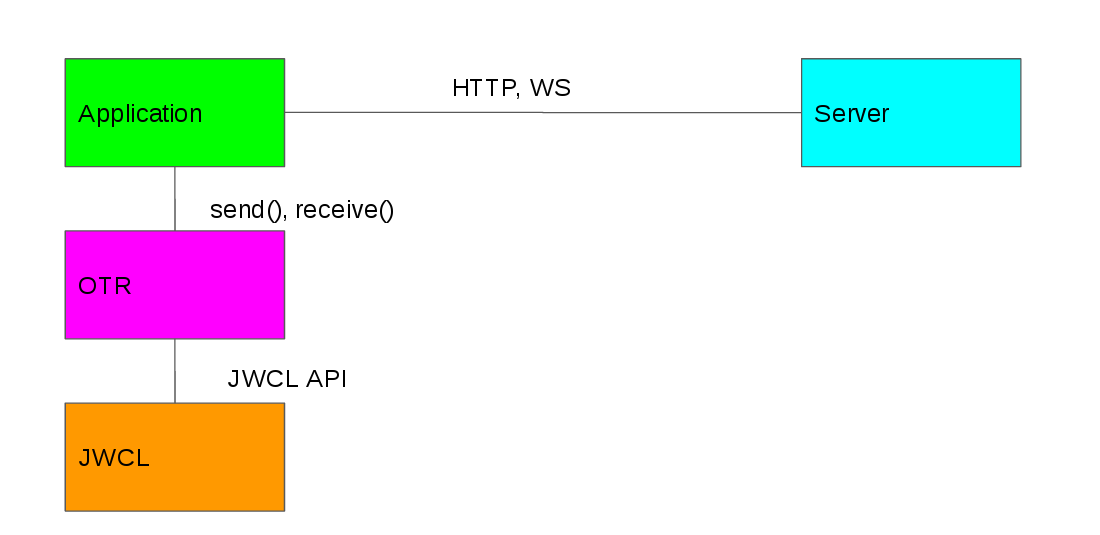
\includegraphics[width=1\textwidth]{architecture.png}
    \caption{Implementation Architecture}
    \label{fig:architecture}
\end{figure}


\section{Application Server}


The application server was written in Python. Flask was used for the web application framework \cite{flask}. Flask Sockets was used to add websocket support to Flask \cite{flask-sockets}. PyCrypto was used for the server side crypto library \cite{pycrypto}.


The application was written as a single page web application so there is only one url that user visits and that is /. This loads the entire application into the user's browser. To support the single page application there are 3 api endpoints that the client application uses to communicate with the server, /api/login, /api/signup, /socket.


\subsection{/api/login}


This endpoint is used for authentication. 


\subsubsection{Success Flow}


The client sends the username and password to the server. The server then looks up the user record in the database by username. The server then compares the salted hash of the provided password with that of the password stored in the database. On success, the server generates a json web token encoding the username and returns the token to the client with status code 200.


\subsubsection{Error conditions}


There are two points of failure possible in the authentication workflow. These are the user does not exist in the database or the user does exists but has provided an incorrect password. According to OWASP's authentication guidelines "An application should respond with a generic error message regardless of whether the user ID or password was incorrect. It should also give no indication to the status of an existing account" \cite{owasp-auth}. This is fulfilled by returning an empty response body and status code 400 in both of these error conditions. This provides no information to the client on whether the failure was the user did not exist or the password was not correct. 


\subsection{/api/signup}


This endpoint is used for registration.


\subsubsection{Success Flow}


The client sends the username and password of the desired account to the server. The server first looks to see if the user already exists in the database. If the username is still available a random 8 byte salt is generated and the users provided password is salted and hashed. A record for this new user is created in the database with the password field holding the salted and hashed password, a websocket field initialized to null, and a public key field initialized to null. An empty body with the response code 200 is returned to the user indication successful creation of the user.


\subsubsection{Error conditions}


The signup flow has only one error condition and that is user already exists in the database. In this case the record is not added to the database and an empty response body with the status code 400 is returned.


\subsection{/socket}


This endpoint is used for websocket communication.


\subsubsection{Success Flows}


This endpoint has two workflows, registration and messaging.


To start, the websocket receives the JSON data from the client. The first step is to get the JWT from the token field in the message. Validation is performed on this token before any further action is taken by the server. After successful validation of the token, the action field determines whether this is a registration or messaging interaction with the server.


If the action is equal to "register" the registration workflow is started. The username stored in the JWT is used to retrieve the user record from the database. The websocket field is set to the current connected websocket instance. This is the purpose of the registration action, to determine what user has connected on what websocket instance so messages can be properly forwarded to the desired recipient rather than broadcasting them. The public key from the data is stored in the public key field. This is used as the long term public key in the OTR protocol. All the active users are informed of the online status of this newly registered user. This is done by sending update messages to all the connected clients not currently registering. The currently registering client receives a register response with the list of current current users and their online/offline status as well.


If the action is equal to "message" the messaging workflow is started. In this workflow the "to" field of the data is checked to determine who to send this message to. The recipients websocket instance is retrieved from the database and the message is forwarded unchanged, with the exception of deleting the JWT token from the message, as this is used for authentication with only the server and should remain private.


\subsection{Error conditions}


This endpoint has three points of failure in the two workflows. The first two have to do with authentication. If the user doesn't provide a token the error message "auth no token" is returned. If the user's token does not validate the error message "auth invalid token" is returned. The third error is in the messaging workflow. If a user attempts to send a message to a user that is not online the error message "unavailable" is returned.


\subsection{Database}


The "database" used in this application is a python dictionary data structure. This database is stored in memory and is wiped every time the server is restarted. This decision was made for simplicity of implementation, development workflow, and needing no dependencies. 


\subsection{Hash Function}


The function used was PBKDF2 with the provided parameters of 10,000 iterations, 16 byte generated key size, and SHA256 as the internal hash function \cite{pkcs-rfc}\cite{dsa-rfc} These parameters were chosen based on RFC 2898's recommendation. In this RFC they recommend a minimum of 1000 iterations and 8 bytes for the salt. 10,000 iterations were chosen as it did not degrade user experience but it does add 10x computation to each hash for an attacker from the minimum recommended value. An 8 byte salt was chosen in conformity with the recommendation. SHA256 was chosen as the hash function as OWASP's guide on using PBKDF2 says that SHA1 is acceptable for now but a more complex hash function may be needed in the future so the decision was made to use a more complex hash function now \cite{owasp-pbkdf}.


\subsection{JWT Implementation}


For the JSON Web Tokens (JWT), RFC 7519 was followed to implement basic functionality \cite{jwt-rfc}. Two functions were implemented to provide this functionality, encode and decode.


\subsubsection{Encode}


To create the token the header which holds the algorithm name used to HMAC, in our case SHA256 and the type which is set as "JWT" is base64 url safe encoded. Then the payload which is a parameter to this function is base64 url safe encoded as well. The concatenation of the header and payload is then HMAC'd using SHA256 as the hash function and a randomly generated server side key as the signing key. The header, payload, and signature are concatenated by using the "." character as the delimiter. This token is then returned to the caller.


\subsubsection{Decode}


In decode split is run on the "." character to get a list of the three parts of our token, header, payload, and signature. First all the values are base64 decoded so that the raw data is available. The signature is then verified by recomputing the HMAC using the same server side key and making sure it is the same as the provided signature. On success, the payload is returned to the caller of the function. On failure, null is returned to the caller signifying failure of the decoding process.


Since this application is running as one instance and one service, symmetric key signing with the HMAC function was used. 


\section{Application Client}


The application client was written in Typescript and compiled targeting ES6 syntax. The application has no dependencies. The client was built as a single page application, so after initial page load the only communication with the server is through the above API's that the server provides. Since these are all JSON encoded messages the application handles all of the UI creation and updates.


There are two states the application can be in, login and chat. On page load, an instance of the OTR class is constructed and placed it in the global data store. A check of the global data store for a JWT is then done. If a token exists, chat is loaded, otherwise login is loaded.


The login state displays a login form prompting the user for a username and password combination. The user can enter their credentials and attempt to login. 


On successful authentication with the server, the response body contains a JWT and the status code is 200. In this case, the username and token are stored to the global data store. After this is completed a long term public private key pair are generated to be used by the OTR protocol. This key pair is also stored in the global data store. After this is complete the application shifts to the chat state.


On authentication failure, which is determined by a response code other than 200, a response to the user is generated by placing the message "Invalid username or password." below the login form. 


The chat state displays a simple chat interface. The user can view the available contacts and their status, the user can then send messages to these contacts. 


A lot happens when the chat state is loaded. 


First a websocket connection with the server is opened. When this connection is successfully opened a "register" message is sent to the server containing the JWT and the public part of the public private key pair. 


Then a listener is added to the websocket instance to be run on any received messages. This listener first parses the JSON data received from the socket. The first check is for an error message in the data, if this exists the error message is displayed to the user and the function is returned from. If there is no error, the action field of the message is looked at. 


There are three actions the server can respond with register, update, and message.


Register and update are actually synonymous for the actions they provide as of now, but the decision was made to keep them as separate actions since they really are distinct behaviors and future work may need support of separate actions for so this was built in with that in mind. The action they do provide is to update the contact list. They receive a contact list from the server, first this list is stored in the global data store. After this, it is displayed to the UI showing the user which users exists in the system and their online/offline status.


The message action is actually a wrapper around the OTR receive function. This action just passes the message along to the OTR receive. After the OTR receive function returns, there is a check if the message contains any plaintext. If this is the case, the message is displayed to the user interface.


When the user goes to send a message they type in the desired recipient and the message text.
A message object is created that has the fields, action, token, from, to, and text. The action is set to "message", token to the JWT, from to the sender's username, to is set to the provided recipient's username, and text is set to the plaintext. This message is then passed to the OTR send function. After the OTR send function returns, the message is serialized and sent to the server to be forwarded along to the recipient.


One question that has not been answered in this section is why OTR send and receive functions are called on all of our messages? The goal of this application design was to separate the cryptographic operations from the functionality of the messaging as much as possible. This is hard to keep completely separate, for example the creation and publishing of the long term public keys is handled in the application. Yet, the messages are passed to the OTR send and receive to be modified. The OTR instance acts as middleware for the application handling all of the cryptographic operations and allowing the application to focus on sending and receiving messages. This design allowed for these two pieces to be developed in parallel and completely separate from each other. If you were to comment out these two function calls the application would function still be a fully functional chat application just without OTR. A lot of information is passed from our applications global state into the OTR send and receive functions so they can perform the operations they need to. The websocket, token, contact list, username, and long term public private key pair are all passed to these functions. What these functions do with all of this information and how these functions operate is covered in the following section.


\section{OTR}


The OTR implementation was written in Typescript and compiled targeting ES6 syntax. The only dependency the OTR implementation has is the JWCL wrapper that will be covered in the next section. This implementation consists of seven main stateless functions that implement each step in the OTR protocol and an OTR class that implements the OTR state machine for a conversation. 


All seven of of these stateless functions have the same function signature that consists of three parameters, local, network in, and network out. All functions return void, any errors are delivered by throwing the corresponding exception. Local, is a data store that stays on the client, this is used for holding keys and other client side data. Local is not a data store for the state though, this is held in the OTR class that will be covered later in this section. Network in, is a read only data structure that is the input to the function coming from the network. Network out, is a passback parameter that is used to return the data that should go on the network after returning from this function. The decision to use separate parameters for input and output was because of the way javascript passes values. Javascript is a pass by reference language. Therefore modification of a variable passed in will be seen by that pointer in the calling function. The issue with that in this case is that the network variable must be kept clean by deleting the old data before adding new data to that object. It was much easier to instead treat the input as readonly and then instantiate a new object for the output that was then written too.


For the following sections describing the authenticated key exchange implementation, the case that Bob is initiating an key exchange with Alice and then sending her a message will be made. Bob and Alice are assumed to both have long term public keys called pubB and pubA that are published and available to each other. In this implementation, that is handled by the application layer as mentioned in the previous section.


\subsection{Authenticated Key Exchange State 1}


In this state Bob starts by generating a random key that will be called R. Bob then generates an ECDH key pair called GX. The public part of GX is encrypted using R as that key, that value will be called aesGx. The public part of GX is also hashed using SHA256 that value will be called hashGx. Bob stores R and GX in his local storage. Bob also places GX in his key storage as his current key pair with Alice. Bob then generates his next key pair for the conversation and stores that as well. The network out object type field is set to "ake1". The aesGx and hashGx fields of network out are set to the their corresponding values.


\subsection{Authenticated Key Exchange State 2}


In this state Alice starts by generating an ECDH key pair called GY. Alice stores GY in her local storage. She then stores the received aesGx and hashGx as well. Just like Bob, Alice places GY in her key storage as the current key pair and generates her next key pair. The network out object type field is set to "ake2". The gy field of network out is set to the public part of GY.


\subsection{Authenticated Key Exchange State 3}


In this state Bob takes GY from the network in object. Bob uses GY and GX to derive random bits called S. Bob uses S to derive two encryption keys called C and C' and four mac keys called M1, M1', M2. and M2'. This process is completed by hashing S in various ways. Next the value MB is created. First an object consisting of four fields, gx, gy, pubB, and keyIdB is created. Gx is set to the public part of GX. Gy is set to the gy received from Alice. PubB is set to Bob's long term public key. KeyIdB is set to 1 as this is Bob's first key with Alice. This object is MAC'd with the key M1 to create MB. Next the object XB is created which consists of three fields pubB, keyIdB, and a value called sigMb. SigMb is computed by signing MB using pubB. Next XB is encrypted using C to get the value called aesXb. Then aesXb is MAC'd using M2 to get the value called macAesXb. The six keys generated as well as Alice's GY are placed in the local storage. The network out type field is set to "ake3". The field R is set to the value of R generated during ake1. The fields aesXb and macAesXb are set to their corresponding values.


\subsection{Authenticated Key Exchange State 4}


In this state Alice takes R from network in. She uses this to decrypt aesGx sent to her by Bob in ake1. Alice then hashes GX and compares the hash to the one that was sent. If this comparison fails an exception is thrown with the message "Error ake4: hashes do not match". If the comparison is a success Alice uses GX and GY to derive the same random bits for S as Bob did. She then hashes S in various ways to get the same six keys Bob computed. Alice first uses M2 to verify the MAC of aesXb. If this verification fails an exception is thrown with the message "Error ake4: mac does not verify". If this verification is successful, XB is then decrypted using C. Alice reconstructs MB by signing the same values as Bob did with M1. Alice then takes pubB and uses it to verify the signature of mB. If this verification fails an exception is thrown with the message "Error ake4: signature does not verify". If this verification succeeds Alice has now validated all of the information Bob sent in ake3. The next step is to send very similar object back to Bob. First MA is computed which is the MAC using M1' of gx, gy, pubA, and keyIdA. These are set to the same values as the were for Bob with the exception if pubA being Alice's instead of Bob's long term public key. XA is again computed in a similar fashion as Bob computed XB. Alices creates the object with the values pubA, keyIdA, and the signature of MA using pubA. Alice encrypts XA using C1' to get aesXa. Alice then MAC's aesXa using M2' to get macAesXa. Alice stores the keys computed from S and GX in her local storage. She also sets their key id field to the keyIdB Bob sent. She then stores GX in Bob's key storage. The network out type is set to "ake4". The fields aesXa and macAesXa are set to their corresponding values.


\subsection{Authenticated Key Exchange State 5}


In this state Bob performs the verifications that Alice did in the first half of ake4. First Bob verifies the MAC of aesXa. If this verification fails an exception is thrown with the error message "Error ake5: mac does not verify". If this verification succeeds XA is retrieved by decrypting aesXa. MA is then computed by using M1' to MAC the same values that Alice did which were gy, gx, pubA, and keyIdA. After this Bob uses pubA to verify the signature of MA. If this verification fails an exception is thrown with the error message "Error ake5: signature does not verify". If this verification succeeds, Bob then sets his key id field to keyIdA and stores GY in Alice's key storage. If all of these verifications succeed the authenticated key exchange is complete.


\subsection{Exchange Data State 1}


Now that the key exchange is complete Bob can send his message to Alice. Bob gets the plaintext from the message passed in by the application layer. Bob takes out Alice's public key and his private key they agreed upon in authenticated key exchange, from his key storage. Bob then uses this public private key pair to derive random bits again called S. He then hashes S in various ways to get four keys sendAesKey, recvAesKey, sendMacKey, and recvMacKey. Bob uses the sendAesKey to encrypt the plaintext to ciphertext. He then constructs an object called TA that has the send key id, the receive key id, the next dh key Bob wants to use, and the ciphertext. Bob then uses the sendMacKey to sign TA getting the value macTA. Bob sets the type field to "ed1" and sets ta and macTa to their corresponding values.
 
\subsection{Exchange Data State 2}


Alice has received Bob's message now and wants to see what it says. She starts by getting TA and macTA from the network in variable. Using the receive key id Alice pulls out her corresponding private dh key and using the send key id she gets Bob's public dh key from her key storage. Alice then uses this public private key pair to derive random bits called S. She then hashes S in various ways to get the same four keys as Bob sendAesKey, recvAesKey, sendMacKey, and recvMacKey except they are flipped. Alice's receive is Bob's send. Alice uses the recvMacKey to verify macTA. If this verification fails an exception is thrown with the error message "ERROR ed2: mac does not verify". If this verification is successful, Alice uses the recvAesKey to decrypt the ciphertext and get the plaintext. She places this in her local storage for the application layer to display.


\subsection{OTR Class}


The OTR class is the go between that lets the application talk to the OTR functions. The class also has the responsibility of running the OTR state machine for each conversation. 


The constructor takes no arguments and creates an empty conversations object. The conversations object is a key value mapping between the username of recipients and their corresponding conversation information. There are two functions that the OTR class has which are send and receive. They both take the same list of parameters which are ws, token, contacts, username, longKey, message. Ws is the websocket connection. Token is the JWT. Contacts is a list of all the active user objects in the system. Username is the username for the active user. LongKey is public private key pair for the active user. Message is the message object being passed in from the application. The message object has the fields action, token, from, to, and text. The send and receive functions in this class add one field to the message object called otr, this holds all of the otr information from the ake1-5 and ed1-2 network out parameters. So how this is related to the function signatures of each of our states mentioned above is as follows. The conversations objects mapping is used as the local store, the otr object is the receiving case is the network in object, the otr object in the sending case is set to the network out object.  


\subsubsection{send}


The send function has two cases to handle, which are a new conversation and a continuing conversation.


In the case of a new conversation, a mapping needs to be created in the conversations object between the recipient's username and relevant information. Key management information is created which is described in detail in the next section. The text of the message is buffered for use after the authenticated key exchange is completed. The otr variable is created with the type field being set to "query". This is a request to start the authenticated key exchange.


In the case of a continuing conversation ed1 is called to encrypt the message. The the otr variable is set to the network out result of the function call. 


A new message object is created with the fields action, token, from, to and otr. Action, token, from, and to are set to the identical fields from the message object that was passed in. Otr is set to the otr object that was created. This object is returned back to application to actually be sent.


\subsubsection{receive}


The receive function has six cases to handle, which are based on the type of message that is received. These are "query", "ake1", "ake2", "ake3", "ake4", and "ed1".


In the case of the type being "query" the otr variable is taken from the message coming in. This becomes the network in variable for the function call to ake1. The otr variable is now set to network out. This is where the websocket that was passed in to this function comes into play. The receive function actually sends a response on behalf of the user. This makes it transparent to the application that the key exchange is taking place. The response has the same action as the message, the token is set to the passed in token, from is set to the username, to is set to the from field in the passed in message since this is a response. Finally otr is set to the otr value that was saved after the completion of the ake1 function call.


In the case of the type being "ake1", "ake2", "ake3", "ake4" the same process is followed. The otr variable is pulled from the received message to be used as the network in value. The next step in the authenticated key exchange is called and the resulting network out is sent as the otr variable in the outgoing message.


For the cases of receiving "ake3" and "ake4" the message buffer that was created in the initial send is checked. If there is a message in the buffer this message is encrypted by calling ed1 and sent as well. 


In the case of the type being "ed1", ed2 is called on the received information to decrypt the message. The plaintext is added to the message data structure and passed up to the application for display to the user.


\subsection{Key Management}


Key management in the OTR implementation is handled by a few variables. They were referenced above as the key store. This section explains how this store operates and explains the process of cycling keys. The OTR class's representation of a conversation has six fields that relate to key management, these are ourLongKey, ourKeys, ourKeyId, theirLongKey, theirKeys, and theirKeyId. 


The ourLongKey and theirLongKey are the long term public private keys that are used during the key exchange. 


The ourKeys, ourKeyId, theirKeys, and theirKeyId are much more interesting. This is the key store for the ECDH key pairs. Our keyId is initialized to be 2 since two keys were generated in either "ake1" or "ake2" depending on which side of the authenticated key exchange our side was. When "ed1" is entered the key ourKeyId - 1 is pulled from ourKeys for use as the private key in the computation of S as described in the ed1 section. The key ourKeyId is pulled from ourKeys for use as the nextDh key. The receiving side is where key rotation takes place. There are two cases that cause a key rotation. The first is if the recvKeyId is equal to ourKeyId, that means ourKeys has no new keys to send so one must be generated. First the oldest key is deleted, then a new dh key is generated and placed in ourKeys, and finally ourKeyId is incremented by one to reflect this process. The second state that causes key rotation is when sendKeyId equals theirKeyId, in this case the nextDh they send us is added to their keys and theirKeyId is incremeneted by one to reflect this change.


\section{JWCL}


JWCL was written in Typescript and compiled targeting ES6 syntax. JWCL is a wrapper that makes the native Web Crypto API easier to work with. JWCL's interface was modeled after SJCL \cite{sjcl-library}. JWCL injects one top level variable, creatively named jwcl, into the global scope. JWCL uses base64 encoding heavily to ensure portability over a network. A result of this is  that raw JWCL output data is not usable by other cryptographic libraries without careful decoding. The jwcl variable has one top level function called random and four modules utils, hash, cipher, and ecc. Utils provides helper functions to translate between binary data, base64 encoded strings, and numbers. Hash provides access to SHA1 and SHA256 functions, and an HMAC class. Cipher provides access to an AES class. ECCprovides access to ECDH and ECDSA classes. JWCL uses classes when the cryptographic primitive needs to maintain state and functions when it does not. For example AES was implemented as a class so the key could be remembered between function calls but SHA1 was implemented as a function because there is nothing to be remembered. 


\subsection{jwcl.utils}


The utils module is focused on providing helper functions for type conversions between binary, string, and integer data types. These can be called from outside the library but their main use is internal. There are eight functions in utils, btos, stob, itob, btoi, btob64, b64tob, stob64, and b64tos.


Btos and stob convert between strings and binary data. Javascript now represents binary data in TypedArrays \cite{mdn-typedarrays}. TypedArrays are not portable over a network so a string representation was needed. This was accomplished by using a Uint8 TypedArray. To go from binary to string an empty string was created. Then the array was looped through. At each byte String.fromCharCode was called to convert the numeric representation of the data to its corresponding character representation \cite{mdn-charfrom}. This worked well with the Uint8 type because the max value for an unsigned byte is 255 and that is well within the capabilities for fromCharCode to convert. This converted character was then appended to the string. Once all members of the array had been converted the resulting string was returned. Stob works the same way just in the opposite direction. First an empty Uint8Array was created with a length equal to the string length. Each character in the string was looped through and string.charCodeAt was called to convert the character back to its numeric representation \cite{mdn-charat}. Once all characters have been placed in the array, the array is returned.


Itob and btoi convert between binary data and integers. At the time of this implementation there was no way to do math with TypedArrays. These functions support up to 32 bit unsigned integers. Itob works by creating a Uint8Array to hold the result. Each of the four bytes is then filled in by taking the floor of the division of the number and 2 to the power of bits were at and then repeating with the remainder. For example 259 would be divided by $2^{24}$ first resulting in 0 so that would go in the high byte. Then $2^{16}$, again 0 in the next byte. Next $2^8$ which would result in 1 remainder 3 so one would go in the second to last byte. Finally 3 is divided by $2^0$ so 3 goes in the low byte position. This array is then returned. Btoi works in reverse. First a total is initialized to 0. Each byte in the array is multiplied by its respective power of two and then added to to the total. This total number is then returned.


Btob64, b64tob, stob64, and b64tos all use the native window.atob and window.btoa functions \cite{mdn-base}. These functions provided base64 encoding. This is used to ensure url and network safe strings for passing data over a network connection. Btob64 first converts the binary data to a string using btos, after this is done the result is passed into window.btoa to get the base64 encoded string. B64tob works in the opposite way, the base64 string is decoded using window.atob then converted to binary using stob. B64tos and stob64 directly call the window functions window.atob and window.btoa respectively. These were implemented simply to have functions complete this action that matched the naming scheme of the rest of the utility functions.


The utils module is fully responsible for all data type conversions and the rest of the JWCL library makes heavy use of its features.


\subsection{jwcl.random()}


The random function provides generation of cryptographically secure random numbers. The function takes one parameter which is the number of bytes to generate. A Unit8Array of that length is generated. The Web Crpyto API random function is called with the array as a parameter. The resulting array is encoded using the bto64 function and the resulting base64 encoded string is returned. Because of this encoding scheme these random numbers must be decoded before use in other contexts. The library handles this for any use of random numbers in the API's.


\subsection{jwcl.hash}


The hash module consists of two static functions, SHA1 and SHA256, and one class, HMAC.


SHA1 and SHA256 both take a plaintext string as input and return a Promise of type string as output which is the digest. The output string is computed using the Web Crypto digest function. This function takes a name parameter as a string and a plaintext parameter as a TypedArray. The strings "SHA-1" and "SHA-256" are passed in to represent their respective hash functions. The stob is called to encode the plaintext string into its related TypedArray. The output of the hash function is again a TypedArray so translation to a string is needed. This is done using the btob64 function.


The HMAC class has a constructor that takes the key as string as input. This key should have been generated using the random function. This key is stored in a local variable for use throughout the lifetime of the class. The HMAC class has two functions, sign and verify.


Sign returns a Promise of type string which is the signature. Sign takes one parameter which is the plaintext string to be signed. First the base64 encoded key needs to be decoded and translated to a TypedArray. This is done by calling the b64tob function. Next a Web Crypto CryptoKey needs to be created. The import key function is used to translate the TypedArray representation of our key to a CryptoKey representation. The import key takes four parameters, name, hash, extractable, and usages. The name is set to "HMAC" since that's what this key will be used for. The hash is set to "SHA-256" so that hash function is used in the HMAC. Extractable is set to true. Usages is set to "sign" since that's the action that is being performed in this function. After this is done the Web Crypto sign function is called. This function takes three parameters, name, key, plaintext. The name is set to "HMAC" since that is the signature algorithm this class performs. The key is set to the CryptoKey. The plaintext is set to the TypedArray of the plaintext string that was passed in which is generated by calling the stob function. The result of the Web Crypto sign is a TypedArray. This is translated to its base64 string representation using btob64 which results in the signature.

Verify returns a Promise of type boolean which is whether or not the signature verifies. Verify takes two parameters which are the signature and the plaintext both of type string. The process of creating the CryptoKey is exactly the same as in sign except the action parameter is set to "verify" and not "sign". After this is done the Web Crypto verify function is called. This function takes four parameters name, key, signature, and plaintext. The name is set to "HMAC" since that is the verification the class performs. The key is set to the CryptoKey. The plaintext and signature both came is as strings and this function takes TypedArrays. Since the resulting signature in sign was base64 encoded b64tob is called to translate the signature to a TypedArray. The plaintext on the other hand is a regular string so stob is used. The result of the Web Crypto verify is a boolean and that is what is returned.


\subsection{jwcl.cipher}


The cipher module consists one class, AES.


The AES class constructor takes the key of type string as input. The key should have been generated using the random function. During construction a private internal counter is initialized to zero. AES also has two private internal constants, counter bytes, and block size bytes. Counter bytes is used to determine how many bytes the counter will be. Block size bytes is used to compute the next counter, a process that will be covered later in this section. They are both set to 16 bytes. As long as the underlying AES implementation does not change block size bytes should always be 16. The AES class has two functions, encrypt and decrypt.


The encrypt function takes the plaintext string as input and returns a Promise of type string. The Web Crypto API needs TypedArray input for both the string and counter. These are created by calling stob and itob on the plaintext and counter respectively. Just like in the HMAC class the key must be imported into type CryptoKey. The parameters that differ in this case are the name and usages parameters. For aes the parameter is set to "AES-CTR" to use the AES algorithm using counter mode. The usages is set to "encrypt" since that is the action this function performs. Once this is done the Web Crypto encrypt function is called. This function takes 5 parameters, name, counter, length, key, and plaintext. The name is set to "AES-CTR" because that is the mode chosen for this implementation. The counter is set to the counter that was translated to a TypedArray. The length is set to 128, this is the number of bits in the counter. The key is set to the created CryptoKey. The plaintext is set to the translated TypedArray of the input plaintext. The output of the encryption is another TypedArray that holds the ciphertext. To create the output the next step is to append the counter to the ciphertext as the first block. The counter is then update using the computation of, counter equals counter plus the ceiling of the length of the message in bytes divided by bytes per block. Finally the ciphertext is translated to a bas64 encoded string using btob64 and returned.


The decrypt function takes the ciphertext base64 encoded string as input and returns a Promise of type string. The first step is to translate the base64 encoded string back to a TypedArray using b64tob. Next the counter is separated by removing the first block of the ciphertext. The CryptoKey is created the same way, with the exception of usages being "decrypt" because that is the action this function performs. The Web Crypto decrypt function is called which takes the same five parameters as encrypt except the plaintext is now ciphertext. The values of these are all the same as encrypt except the plaintext TypedArray is replaced with the ciphertext TypedArray. The counter is then updated to the max of the internal counter and the received counter. This is done to keep an instance of AES in sync with another instance across a network. The decrypt function returns a TypedArray for the plaintext so that is translated to a string by calling btos and returned.


\subsection{jwcl.ecc}


The ECC module consists of two classes, ECDH and ECDSA. 


The ECDH constructor takes one parameter which is a key of type eccKey. This type is an object with two fields, public key and private key both of which are strings. ECDH has one static function generate and one function derive. 


The static generate function is used to generate ECDH key pairs. This function was implemented statically so that key generation could be done separately from object construction. This is necessary because key generation is an asynchronous process and object construction is not. This function takes no parameters and returns a Promise of type eccKey. Since the key generation process for ECDH keys is not just generate random numbers and use them, this function is provided. The Web Crypto generateKey function is called. This function takes four parameters name, namedCurve, extractable, and usages. The name is set to "ECDH". The named curve is set to "P-256". This curve is approved for use by NIST for the federal government \cite{nist-curves}.
Extractable is set to true. Usages is set to "deriveBits" so that our key pair can be used to generated random bits. As mentioned in the constructor the eccKey type holds the public private key pair as strings. The process of translating the CryptoKey pair to string is the same for both public and private key. First they key is exported under the Json Web Key format. This format is serialized using JSON.stringify. The string output is then base64 encoded using stob64. This gives a network safe representation of the keys. The public and private key strings are then placed in an eccKey object and returned.


The derive function takes one parameter which is a base64 encoded public key string. This value should come from the public part of the eccKey that was created using generate. This function returns a Promise of type string which is the derive bits. These can be used as a key in the aes and hmac classes or any other place random bits are needed. The process done in key generation first needs to be reversed so the CryptoKey representations of the public and private keys are available. This is again the same for both public and private keys and is done by calling the Web Crypto importKey function. This function takes six parameters, type, key, name, namedCurve, extractable, and usages. The type is set to Json Web Key by the string "jwk". Key is the JSON representation of the key. This is gotten by calling b64tos and then JSON.parse on the result. The name, namedCurve, extractable, and usages are the same as in generate with one important difference. When importing the public key usages is left blank. There is nothing in the Web Crypto API spec that says why this is but the code does not function if this value if set to derive. Once the keys are imported the Web Crypto deriveBits function is called. This function takes three parameters, name, publicKey, and privateKey. Name is set to "ECDH", the public and private Keys are set to their corresponding CryptoKeys. This function returns the derived bits as a TypedArray so they are translated to a base64 encoded string using btob64. The resulting string is returned.


The ECDSA constructor takes one parameter which is of type eccKey, exactly the same as ECDH. Ecdsa has one static function generate and two functions sign and verify.


The static generate function takes no parameters and returns a Promise of type eccKey. This function works identically to that of ECDH with the only exception being the name is set to "ECDSA" during the call to the Web Crypto generate key function.


The sign function takes one parameter of type string as input. This is the plaintext to be signed. This function returns a Promise of type string which is the signature. The first step of sign is to decode the private key from the base64 string to the CryptoKey representation. This is done the same way as in ECDH except name is set to "ECDSA". The Web Crypto sign is then called. This is the same function that hamc uses. This function takes four parameters, name, hash, private key and plaintext. The name is set to "ECDSA". The hash is set to sha256. The key is set to the imported private key. The plaintext is set to the input plaintext translated to a TypedArray. This is done by calling stob on the input parameter. The resulting signature is also a TypedArray so btob64 is called to get the base64 encoded string result. This is returned.


The verify function takes two parameters signature and plaintext and returns a Promise of typed boolean signifying if the signature verified or not. The public key is used for signature verification so that is converted to a CryptoKey in the same way the private key was in sign. Next the Web Crypto verify function is called. This function takes five parameters, name, hash, public key, signature, and plaintext. The name and hash are set to the same values as sign. The public key is set to the CryptoKey representation of the public key. Both the signature and plaintext expected TypedArray so the input must be converted. This is done by calling b64tob for the signature since it was base64 encoded, stob is used for the plaintext. The boolean result of verify is returned.
 
